%
% RING Meeting Template
% Edit and compile with pdflatex
%
% If you absolutely want to use latex to produce DVI, be sure to use only
% compatible graphisms (.eps is the best).
% You can also include .eps figs only and use pdflatex (thanks to epstopdf),
% just check that you have "shell_escape = 1" somewhere in a texmf.cnf file,
% or that you call "pdflatex -shell-escape file.tex".
%
% This template uses natbib.sty bibliography style, so you can use commands
% like \citet{}, \citep{}, \citeauthor{} or \citeyear{}.

%-----------------------------------------
% Template Mode preprint / final:

%\documentclass[preprint]{ring20} 

% Please : submit your paper in the final mode
\documentclass[final]{ring20} 

%% relative path to the graphic folder from the tex file
\graphicspath{%
{./Figures/}%
}

\usepackage[disable]{todonotes}
%\usepackage[]{todonotes}

\newcommand{\bx}{\mathbf{x}}
\newcommand{\bn}{\mathbf{n}}

%-----------------------------------------
% First page information :

\title{Progresses in the implicit structural modeling benchmark}

% Title used for the title over-riding report
% (It may be the same than the main title if small enough)
\shorttitle{Implicit structural modeling benchmark}

% Author(s) name(s) on the first page
\author[1]{Guillaume Caumon}
\author[1,2]{Julien Renaudeau}
\author[1]{Modeste Irakarama}
\author[3]{Lachlan Grose}
\author[5]{Miguel de la Varga}
\author[7]{Michael Hillier}
\author[7]{Eric de Kemp}
\author[5]{Florian Wellmann}
\author[1]{Pauline Collon}
\author[4]{Gautier Laurent}
\author[3]{Laurent Ailleres}
%\author[8]{Who else ? Order to be determined}

%Adresses of the authors (affiliations)  
\affil[1]{RING, GeoRessources / ENSG, Universit\'e de Lorraine / CNRS, France}
\affil[2]{Schlumberger, France}
\affil[3]{Monash University, Australia}
\affil[4]{Univ. Orl\'eans, CNRS, BRGM, ISTO, France}
\affil[5]{RWTH Aachen, Germany}
\affil[6]{BRGM, France}
\affil[7]{NRCan, Canada}

%often used affiliations
%\affil[1]{GeoRessources - UL/CNRS/CREGU, ENSG, Vandoeuvre-l\`es-Nancy, France.}
%\affil[2]{GeoRessources - UL/CNRS/CREGU, ENSMN, Nancy, France.}
%\affil[3]{Centre d'hydrog\'eologie et de g\'eothermie, Universit\'e de Neuchatel, Neuchatel, Suisse.}
%\affil[5]{INRIA - Project Alice, Villers-l\`es-Nancy, 54600, France.}

% Author(s) name(s) used in the footer of each page
\shortauthor{Caumon et al.}

%-----------------------------------------
% The document :
%

\begin{document}
\maketitle

\begin{abstract}

Implicit methods have gained significant popularity in recent years as 
an alternative to surface-based structural modeling methods (also known as 
contouring, gridding or explicit structural modeling). These approaches represent 
geological interfaces as equipotentials of a scalar field. 
Whereas existing formulations share the same principle, they have not yet been 
quantitatively compared beyond theoretical discussions. In this paper, we review 
the main categories of implicit methods and list their parameters. We propose 
three benchmark data sets: a folded turbidite, a carbonate buildup 
displaying large thickness variations and a convoluted synthetic surface 
representing a hydrothermal body. We applied several methods and several 
implementations on these data sets, and provide the chosen parameters for each 
methods. Results are compared in terms of accuracy, ability to predict 
some features not present in the data, and topological complexity. 
Results illustrate the difficulty to come up with a universal geological 
modeling method, and highlight the need to build additional geological 
knowledge and to consider uncertainty in future structural modeling methods.  

\end{abstract}

\todo[inline]{Writing mode: I suggest a ``dictatorial collaborative writing'': co-authors send me comments / paragraphs / figures / results in annotated PDFs, LateX (or Word) format and I will incorporate them in the LaTeX document.

Authors: list and order to be discussed. }


\todo[inline]{Eric: "I was thinking of developing  further a 3d matrix with principal axis indicating model  level of complexity (dimension+properties, geological events, cumulative spatial features) as well as a matrix indicating data complexity (density, number of types, clustering)  . Each test case could fit into these two matrices and could be increased in dimensionality but is at least more intuitive where the case examples fall visually. Each case would get a complexity badge or glyph classifying it."}

\textit{This paper an update from the 2019 RING Meeting version. As compared to last year' version, the introduction has been edited to better frame the objectives, the theoretical review of the methods has been enriched, and the evaluation criteria have been added. Please note that this version of the has not yet been reviewed by all co-authors. Updates will be available at \url{https://github.com/Loop3D/ImplicitBenchmark/tree/master/Paper}.}

\section*{Introduction}

The formation and deformation of rocks at geological time scales generate a large variety of geological structure shapes. Three-dimensional structural modeling aims at reconstructing these structures from spatial samples created from field observations and/or from geophysical images of the subsurface. Historically, structural modeling first meant computing the depth contours of a particular geological interface \citep[e.g.,][]{Walters1969AB,Hardy1971JGR,Briggs1974G,Bolondi1976G}. During the 1990's surface-based models using polygonal or parametric surfaces emerged as a more powerful way to represent complex structures such as recumbent folds or salt diapirs \citep{Mallet1992CD,deKemp1999CG}. However, these explicit modeling approaches are difficult to automate in complex geological settings, and call for various degrees of interactive input to generate the structures. Since then, progress in memory and computational capabilities have led to implicit modeling formulations, in which geological interfaces between rock units are defined by isovalues of a three-dimensional scalar field \citep{Lajaunie1997MG,Cowan2002ASGMEM,Calcagno2008PEPI,Frank2007CG,Caumon2013GaRSITo,Souche20137ECEISE2,Hillier2014MG,Laurent2016MG,Laurent2016EaPSL,Martin2017CG,Grose2017JSG,delaVarga2018GMDD,Irakarama2018EAGE,Grose2019JoSG,Renaudeau2019BEMRMX,Renaudeau2019MG,Manchuk2019CG}.

Implicit modeling provides a high degree of automation even for complex geological shapes, and can also account for various types of structural data such as off-contact orientation  measurements. As a result of these methodological advances, three-dimensional structural modeling is increasingly becoming part of the geologist's toolbox. By integrating sparse data into a consistent graphical model, the promise of computational structural modeling is to help geologists to analyze their data, to develop conceptual interpretive models, and to make subsurface forecasts based on model outcomes. 

Automation of three-dimensional structural modeling is essential to meet these needs effectively, especially when several possible models need to be considered to appropriately characterize subsurface uncertainty \citep{Wellmann2018AiG}. However, ``seeing is believing'', so a risk is that applied geologists believe that a particular structural model is true, whereas it is only determined from the available spatial data (whose reliability may vary) and from mathematical or numerical terms telling what the three-dimensional model should look like away from the data points. Indeed, in general, the data points are not numerous enough to fully characterize the structural geometry, hence the need for some sort of regularization \citep[e.g.,][]{Renaudeau2019MG}. The parameters involved in the regularization term influence the results, but may not be easy to determine by layman users. These parameters oftentimes correspond to abstract mathematical terms (e.g., least-squares weights, variogram ranges, basis function parameters) which can be intuitively translated into model features (e.g., degree of data fit, stiffness of the surface) but not so easily into classical structural concepts, which generally involve a blend of geometric, kinematic, and mechanical reasoning. Analyzing and understanding the results of a particular method can be difficult, as it may call for the practitioner to delve into the theory of partial differential equations, numerical optimization, or geostatistics. Another approach to deal with data ambiguity and uncertainty is to actually consider multiple structural models. However, all structural uncertainty modeling approaches rely on a deterministic structural modeling engine \citep[see ][ and references therein]{Wellmann2018AiG}.

To address these challenges, several authors have proposed to more directly integrate structural concepts into modeling methods \citep{DeKemp2003G,Maxelon2009CG,MassiotGM2010,Laurent2016EaPSL,Grose2017JSG,Grose2018JGRSE,Grose2019JoSG}. This can be achieved either by manually or automatically adding new interpretive ``data'' such as fold hinges, or by integrating new mathematical terms in the interpolation problem. Another recent line of research has been on the mathematical formulation and the discretization of the regularization term \citep{Laurent2016MG,Martin2017CG,Irakarama2018EAGE,Renaudeau2019MG}. In this frame, theoretical comparisons between the various published methods can be made, but they may be of limited use to practitioners. Practical comparisons between method are delicate, because they rely on software packages whose implementation is not necessarily available. The level of implementation descriptions may also vary from one paper to another, making it difficult for graduate students to reproduce previous work. 

In this paper (Section \ref{sec:methods}), we propose a synthetic review of the various interpolation methods which form the basis of implicit structural modeling software. The goal of this presentation is to use consistent notations for all methods, with the intent to more easily highlight similarities and differences between these various methods. We briefly summarize the features and variants of six computer implementations of these methods, and stress the main parameters which can be used to adapt them to a particular geological setting. As in machine learning, tuning these method parameters using validation data can be achieved in principle. However, the general lack of data may entail a poor predictive ability for parameter-rich models (overfitting); conversely, parsimonious models may be more stable but have a lower fit. This may explain why, in practice, parameter tuning is seldom done in three dimensional structural modeling. Another reason is that defining a goodness criterion is not immediate in the case of geological models. Geologists are trained to decide on the quality of a particular model based on their expertise, and are often reluctant to use purely data-driven methods for that. Expressing in mathematical terms the ``geological realism'' of a particular structural model is possible under some conditions, but it can be difficult to automate and, in general, is still an open problem \citep{Caumon2010MG}. 

The above remarks motivate the realization of the present benchmark study, which is the first community effort of its kind in the field of three dimensional structural modeling. To keep this first study tractable, we limit ourselves to three benchmark data sets in various geological contexts. Similar benchmark data exist in the computer graphics community \citep[e.g.,][]{BLNTS13}, but they generally aim at reconstructing only one single manifold surface from a relatively dense point cloud. In geosciences, the difficulty to access the subsurface generally entails more sparsity and more diversity in the field data. In particular, stratigraphic orientations are often available from fieldwork and dipmeter measurements in boreholes. Another difficulty specific to geological modeling is the presence of faults, and the simultaneous reconstruction of several conformable stratigraphic surfaces with just one scalar field, which raises questions about the management of thickness variation \citep{Laurent2016MG}. The data sets presented in this paper (Section \ref{sec:data}) account for these geological peculiarities and propose several test cases of variable complexity. Each case includes basic data types (points and orientations). To keep the comparison simple, more advanced data types such as fold axis, foliation data, and structural lineations are not considered in the present paper. Some faults are present in two data sets because they we observed, but they are local and only have a limited displacement. Considering how the various interpolation methods manage faults is outside the scope of this paper. 

In Section \ref{sec:results}, we propose a set of metrics to compare results, and explain why and how these metrics were selected. The goal of this benchmark is not to provide a general ranking of the various interpolation methods. Rather, the goal is to gain insights about the various methods on a set of specific problems. Indeed, measuring some aspects of the results quality is always useful and may help defining avenues for future research. Whereas a global ranking of methods based on these metrics could be tempting, we do not recommend it, because metrics are incomplete and results obtained are case-specific and non-exhaustive. For example, we deliberately chose in this paper to reflect the current practice of geological modeling by a applying a set of implicit modeling methods without parameter or hyperparameter tuning. Again, we expect that such an application can bring insights about the methods and their suitability to provide a reasonable approximation of three geological domains from incomplete observations. Generalization of the method's performance to other application domains or data configurations should not be taken for granted. For extensibility and completeness, the three-dimensional models obtained with the various codes are available on a public repository \footnote{\url{https://github.com/Loop3D/ImplicitBenchmark/}}. This makes it possible to scrutinize the results, to add new assessment metrics and also to add new modeling results and new data sets in the future. SKUA Macros implementing the proposed analysis metrics and some Jupyter notebooks are also available on the repository to help with the reproducibility of the metrics computation. 

%Software availablility and usability are important, sability issues, even though they can important, but we will focus on  Among these, the ability of a particular interpolation method to interpolate or extrapolate correct structural geometries away from data points can always be challenged. The adequacy of automatic methods has been debated since the early times of automatic map contouring \citep{Walters1969AB}. The data density should be such that results are well constrained.  ideally, a good method should be able produce results similar to those of a skilled structural geologist.  but this can be difficult to quantify.  . In principle, the goodness of an interpolated structural geometry can be measured on a particular data set by cross-validation (ie: computing the error between the forecasted geometry and some randomly chosen data points). However, as in machine learning, the tuning parameters of a particular method can be optimized using cross-validation, raising the risk of overfitting. Philosophically, 

\todo[inline]{
Previous comments: 

PC: "this supposes there is a "reference true" surface? I do not like it very much... 
Shoudn't we  keep the analysis focused on what we know (data, geological concepts ?). 
In this case, I would prefer "ability to consistently extrapolate the surface"... 

MI: "- What is "quality" in this context and how do we measure it?
- About the ability to predict the reference surface away from data, as we discussed some time ago, I think this is questionable.
  In practice, I can think of two cases: (1) Either we have an a priori on that reference surface away from the data  and therefore we should provide that information to our interpolator.
  Otherwise we know in advance that the interpolator will most likely not predict the surface away from the data because we explicitly ask the interpolator for a "smooth" surface.
  (2) Either we do not have an a priori on that reference surface and therefore we just have to accept what the interpolator gives us. In this second case, different interpolators
  might give different results. We can certainly compare and comment on these results but I don't see how we can decide which are "better" since we are in a case of no a priori. " 
}

\section{A review of implicit modeling methods}
\label{sec:methods}

\todo[inline]{GC: I have expanded this section as compared to last year, but not up to a very detailed description of every method. Instead, I have tried to summarize the main ideas and give the key equations. This section may still contains some approximations and errors, and probably need editing to improve clarity by a general readership. Please have a read and comment and don't hesitate to make (constructive) suggestions. } 

We now propose a brief review of the main methods proposed to compute three-dimensional scalar fields in implicit geological structural modeling. 
Consider $S$ as the set of three-dimensional positions {x} where a three-dimensional scalar field $f(\mathbf{x})$ takes the value $f_S$: 

\begin{equation}
\label{eq:levelset}
  S = \{\mathbf{x} | f(\mathbf{x}) = f_S\}.
\end{equation}

In the general case of a spatially variable scalar field $f$, these positions form a two-dimensional manifold surface called iso-surface or level set, which represents geological surfaces in implicit methods. 

The expression (\ref{eq:levelset}) can be extended to represent 
at once a stratigraphic series of $K$ conformable horizons 
$S_1, \ldots, S_K$ using different iso-values $f_1, \ldots, f_K$. 
In the following, we will call $f$ the stratigraphic function, which can be seen 
(in a chronostratigraphic sense) as a relative geological time \citep{Mallet2004MG,Lomask2006G,Wu2012G}.

In the presence of $N_k$ data points at positions $\{\mathbf{x}_1^k, \ldots, \mathbf{x}_{N_k}^k\}$ for the horizon $S_k$, all implicit surface interpolation methods start by forming the following system of equations: 

\begin{equation}
\label{eq:datasystem}
\begin{array}{r c l}
f(\bx_1^1) & = & f_1 \\
\vdots & \vdots & \vdots \\
f(\bx_{N_1}^1) & = & f_1 \\
\vdots & \vdots & \vdots \\
\vdots & \vdots & \vdots \\
f(\bx_{N_1}^K) & = & f_K \\
\vdots & \vdots & \vdots \\
f(\bx_{N_K}^K) & = & f_K \\
\end{array}
\end{equation}

The system (\ref{eq:datasystem}) can be complemented with other data terms corresponding to $N_O$ orientation measurements. These orientations, made at locations 
$\bx_o$, $o = \{1, \ldots, N_O\}$, may take the form of unit strike and dip vectors $(\mathbf{s}_o, \mathbf{d}_o)$ or unit normal vectors $\bn_o$, with $\mathbf{n}_o = \mathbf{d}_o \times \mathbf{s}_o$.  
 
From this information, several methods have been proposed to compute a stratigraphic function at any spatial location $\mathbf{x}$. Essentially, these methods make different choices about the way data are handled, the type of basis function used to approximate the solution, the mathematical formulation to ensure the uniqueness of the solution. These differences have an impact on the way the solution is evaluated and visualized. 
 
\subsection {Data handling}

In most approaches, the scalar field values $f_k$ need to be chosen before the interpolation and are imposed in the interpolation problem \citep[e.g., ][]{Frank2007CG,Hillier2014MG,Renaudeau2019MG}. In practice, these values can be chosen using a rough estimate of the cumulative thickness between each horizon and some reference horizon, or any other convenient value proportional to that cumulative thickness \citep{Caumon2013GaRSITo,Collon2016I}. Orientation information can be integrated either by equating the normal to the scalar field gradient ($\nabla f_{\bx_o} = \mathbf{n}_o$, which  carries information about the stratigraphic polarity and assumes that the interpolated scalar field approximates the signed distance to some reference horizon), or by equating the dot products between the scalar field gradient and strike and dip gradients ($\nabla f_{\bx_o} \cdot \mathbf{s}_o = \nabla f_{\bx_o} \cdot \mathbf{d}_o = 0$, which does not use polarity and does not carry any assumption on the norm of the scalar field gradient). 

To avoid the pre-estimation of the horizon values $f_k$, dual cokriging \citep[DcK, ][]{Lajaunie1997MG,Chiles04OMSMP} performs a substitution in System (\ref{eq:datasystem}) so as to consider (unknown) increments of the scalar field as compared to one reference horizon instead of the absolute isovalues. The primal form of the cokriging system reads

\begin{equation}
\label{eq:DcK}
f(\bx) - f_{ref} = \sum_{o=1}^{N_O} (\lambda_i \bn_o^x + \mu_i \bn_o^y + \nu_i \bn_o^z) + \sum_{k=1}^{K} \sum_{j=2}^{N_K} \lambda_{j}^{k}[f(\bx_j^k) - f(\bx_1^k)], 
\end{equation}

where $f_{ref}$ is an arbitrary value chosen for one of the horizons, $k$ refers to the horizon index, $j$ is the point index on each horizon (up to a permutation), and $\lambda_i$, $\mu_i$, $\nu_i$ and $\lambda_j^k$ are the unknown kriging coefficients. In Eq. (\ref{eq:DcK}), the orientation data $\bn_o$ are treated as secondary data in the estimation of the scalar field. The cross-covariance between the scalar field and its gradient and the covariance of the gradient, are determined analytically from the chosen covariance function. For the problem (\ref{eq:DcK}) to be well-posed, at least one orientation data point must be available. 

Other possible data that have been integrated in the interpolation system relate for instance to tangent data \citep{Lajaunie1997MG, Caumon2013GaRSITo, Hillier2014MG}, fold axis \citep{MassiotGM2010,Hillier2014MG}, fold vergence \citep{Laurent2016EaPSL,Grose2017JSG} and layer thickness \citep{Laurent2016MG}. For the sake of brevity homogeneity of the application, we do not cover these additional data types in this paper. 

\subsection{Basis functions} 

The data terms described above only provide information at data location. To evaluate, process or visualize the scalar field everywhere on a computer, numerical methods rely on the general formulation 

\begin{equation}
\label{eq:basis}
  f(\mathbf{x}) = \sum_{i=1}^{N}{v_i\varphi_i(\mathbf{x})},
\end{equation}
\noindent where $v_i$ are some coefficients and $\varphi_i(\mathbf{x})$ some basis functions \citep[e.g., ][]{Hillier2014MG,Renaudeau2019MG,Wellmann2018AiG}.
 
In radial basis function interpolation \citep[RBF, ][]{Carr2001,Cowan2002ASGMEM,Hillier2014MG} and in the dual co-kriging, the basis functions (or covariance functions)are centered on the data points, and a global polynomial term is often considered to capture the overall trend over the domain. In this case, $N$ is equal to the total number of data points plus the number of terms $N_P$ of the polynomial ($N = N_P + N_O + \sum_{k=1}^{K}{N_k}$). In both cases, the choice of the basis function will govern the shape of the iso-surfaces of the interpolated scalar field. As opposed to classical applications of Kriging, inferring the type and parameters of the covariance function from the data is difficult by the non-stationarity and the increment formulation. Therefore, the choice of the covariance function is mainly heuristic, with the mathematical requirement that the covariance function must be twice differentiable to compute the covariances $Cov\left(f(\bx), \nabla {f}(\bx+\mathbf{h})\right)$ and $Cov\left(\nabla f(\bx), \nabla f(\bx+\mathbf{h})\right)$. 

In this study, we use the code GemPy \cite{delaVarga2018GMDD} which implements DcK, and uses the cubic covariance function for its  robustness and its ability to provide coherent results in many studies: 

\begin{equation}
C(r) = \begin{cases}
C_0(1-7(\frac{r}{a})^2+ \frac{35}{4}(\frac{r}{a})^3
- \frac{7}{2}(\frac{r}{a})^5 +\frac{3}{4}(\frac{r}{a})^7) &
\text{for } 0  \leq r \leq a \\
0 & \text{for } r  \geq a
\end{cases},
\end{equation}

where $r$ represents the distance between the points (e.g., between the position $\bx$ to estimate and the data point $i$ in Eq. (\ref{eq:basis})), $a$ is the range (the maximum influence distance of a data point) 
and $C_0$ the variance of the data. In GemPy, it is recommended to choose a range value close to the
maximum model extent avoids mathematical artifacts in the solution. There is no strong guideline 
to choose the values of the covariance at 0, as changing this value only weights the relative influence of the values and of the gradient data, hence does not affect the shape of the isosurfaces. As in classical kriging, it is also possible to add a nugget effect to the covariance function to transform the exact interpolation as an approximation. In this case, the nugget value relatively to $C_0$ controls the degree of approximation (exact if zero, polynomial if equal to $C_0$. This feature is used in two other codes used in this study: SurfE \citep{Hillier2014MG} and MSS {\citep{Renaudeau2019MG}. 

The SurfE code \citep{Hillier2014MG}, used in this study also implements the increments interpolation approach. It allows for testing many different types of basis function. When applying SurfE to the benchmark data sets, we tested the cubic basis function 
\begin{equation}
\varphi_{C}(r) = r^3
\end{equation}
and a multiqudric basis function
\begin{equation}
\varphi_{MQ}(r) = (\epsilon^2 + r^2)^{3/2},
\end{equation}

where $\epsilon$ controls the flatness of the basis function as the distance $r$ increases. 

In discrete smooth interpolation \citep[DSI, ][]{Frank2007CG,Caumon2013GaRSITo,Souche20137ECEISE2,Laurent2016MG,Irakarama2018EAGE}, the number of basis functions $N$ refers to the number of nodes of the mesh used to approximate the solution. In tetrahedral formulations, each basis function $\varphi_i$ is a piecewise linear ``hat function'' (equal to 1 at node $i$, linearly decreasing on the tetrahedra surrounding node $i$ and equal to zero at all the other nodes). These basis functions imply a piecewise constant gradient of the scalar field. They are used in two codes used in this study: StructuralLab \citep{Frank2007CG,Caumon2013GaRSITo} and LoopStructural. 
In the SIGMA code \cite{Irakarama2018EAGE}, Lagrange polynomials defined on a Cartesian grid are used to discretize the data. The basis functions which control the smoothing term are estimated using finite differences operator. LoopStructural and MSS also implement some finite difference operators, for which the type of basis function is not explicitly defined. 

As recently discussed by \citet{Renaudeau2019MG}, the choice of the basis function used have a strong impact on the structure of the linear system that needs to be solved to evaluate the coefficients $v_i$ in Eq. (\ref{eq:basis}): a relatively small but dense system is formed in the case of RBF and DcK, whereas a larger but sparse system is formed in the case of piecewise linear DSI. Recently, \citet{Renaudeau2019MG} and \citet{Manchuk2019CG} proposed to use moving least squares (MLS) polynomial basis functions centered on some interpolation points. As MLS functions have a local support, data points only influence a finite number of interpolation points, and the solution does not explicitly depend on a mesh. This is the main approach used in the MSS implementation code. 

\subsection{Mathematical principles} 

Although the problem is the same to the various existing methods, several mathematical frameworks have been proposed to derive the interpolation systems and to ensure the uniqueness of the solution. 
All methods rely to some extent on optimization (or constrained optimization) and generalized regression to interpolate or approximate the scalar field. Classically, kriging estimates the unknown value as a linear combination of surrounding known values, see Eq. (\ref{eq:DcK}). The coefficients then depend on the chosen variogram model and are obtained by minimizing the estimation variance under the unbiasedness condition. Dual kriging is based on a rewriting of the kriging estimator in the same form as (\ref{eq:basis}), which calls for explicitly inverting the covariance matrix \citep{Lajaunie1997MG,Chiles04OMSMP}. The form of that system is similar to that of RBF interpolation \citep{Dubrule1984CG,Hillier2014MG}. The latter is obtained by applying (\ref{eq:basis}) to all data points, under the constraint that the solution should be orthogonal to the polynomial term \citep{Carr2001,Hillier2014MG}. In the DcK and RBF systems, the number of unknowns is such that the problem is well-posed, possibly BY adding Lagrange multipliers. It should be noted that the RBF solution can, in some cases, be efficiently approximated on a discrete Cartesian mesh by a simple iterative algorithm \citep{Park2006ITVCG}. 

In DSI, the solution is obtained by a weighted least-squares formulation made on the mesh-based basis functions (\ref{eq:basis}). All variants of DSI write the data term (\ref{eq:datasystem}) for the chosen mesh. As the number of mesh nodes is generally larger than the number of data, a regularization term is based on a minimization of the local variation of second derivative of the scalar field $f$. Several quantities representing this second derivative have been proposed, for instance: the minimization of the gradient difference between two adjacent tetrahedra \citep{Frank2007CG}; discrete Laplacian \citep{Irakarama2018EAGE}; sum of one-dimensional second derivatives approximated along several directions using finite differences \citep{Irakarama2018EAGE}; thin plate bending energy discretized with MLS polynomial basis functions \citep{Renaudeau2019MG}. Note that, although DSI in implicit modeling is often assimilated to the constant gradient regulatization in piecewise linear tetrahedra, its formulation allows for many other regularization possibilities \citep{Mallet1992CD}. Indeed, it starts from a graph-based representation of the mesh nodes and considers a class of general linear combination from nodes neighborhoods to ensure convergence. Alternatively, it is possible to use the same approaches as for solving partial differential equations, for instance the finite element method (FEM). Data then play the role of boundary conditions and the continuous energy formulation to be minimized, plays the role of the regularization in DSI \citep{Renaudeau2019MG}. In both cases, an important parameter is the weight penalizing the regularization term against the data term in the least-squares system. 

Although they may belong to different conceptual frameworks, two modeling methods can be shown to be equivalent in some specific case. For instance, choosing a linear RBF is equivalent to minimizing the isotropic biharmonic thin spline energy \citep{Carr2001}. This relates to some basis functions corresponding to the fundamental solutions of some partial differential equations. Similarities between some DSI formulations and continuous energy formulations have also been highlighted \citep{Renaudeau2019MG}. However, comparisons are made difficult by the diversity of variants which have been proposed within each class of methods. The correspondence between the various method parameters is difficult to establish. Implicit or explicit criteria about the mathematical quality and rigor of a particular approach may be defined, but they do not necessarily correspond to the experience of practitioners, which also depends on experience, user interface and the ability of a particular implementation to effortlessly produce a model deemed geologically realistic. This is challenging in itself, as the above method are clearly data-driven, and none pretends to explicitly represent the succession of geological processes which actually generated the structures \citep{Caumon2010MG,Jessell2010T}. This calls for better understanding what controls the model shape away from the observations in the various approaches. The goal of this paper is to provide some benchmark data forming a first basis for such practical comparisons on some relatively challenging geological data sets. 

% In most structural modeling software implementing the above methods, parameter default values are generally chosen using heuristics. One of the goal of this benchmark is to assess the method's behavior on a set of common data set using these default parameter values to gain insights in these particular settings. Future applications may also include parameter tuning. However, most codes allow practitioners to change these parameters by trial-and-error to adapt the modeling results based on data quality and on the geological context. This confers a strong importance to subjective expert judgment of the quality of the solution.  %As none of the above methods directly models the geological processes which generated the structures of interest, we can paraphrase George Box in acknowledging all these models are wrong, but that they are useful in practice. Their existence and their diversity reflects the various types reasoning used to approach, understand and quantify geology.

\subsection{Spatial discretization}.

DcK and RBF are meshless approaches, in the sense that the solution has a high degree of smoothness and can be evaluated everywhere in space without the need for filling the domain with a mesh. Once the system has been solved, the evaluation for a given position is given directly by Eq. \ref{eq:basis}. It only involves to compute the distance between the evaluation point and the data points. For visualization and further processing, the solution is generally evaluated at the vertices of a Cartesian grid or unstructured mesh. Increasing the spatial resolution of that visualization mesh only increases linearly with the number of evaluation nodes. However, adding new data calls for globally updating the interpolation, which calls for efficient solvers such as the fast multipole method \citep{greengard_fast_1987}. 

In mesh-based methods the computation is made on the discrete support at the same resolution as the visualization. Adding a stratigraphic data can be made efficiently by recomputing the solution locally, as the basis functions have a local support. Visually, coarse meshes may display some discontinuites of the first derivative of the scalar field. Increasing the changing the of the modeling support calls for solving the interpolation problem again, unless the mesh change is local \citep{Frank2007CG}. 

As meshes can be difficult to generate, the above remarks may suggest that the meshless methods are always preferable. However, the ultimate goal of a geological structural model is generally to simulate fluid flow, deformation or other physical quantities in the subsurface. Unless meshless techniques are also used in these simulations, meshing complexity will, therefore, step in. This even holds for model visualization, as the visualization implicit geological surfaces is generally achieved on discrete meshes by polygonal isosurface extraction algorithms such as the marching cubes \citep{Calcagno2008PEPI} or marching terahedra method \citep{Frank2007CG}. \todo[inline]{Did anyone try ray tracing with meshless approaches ?}

\subsection{Summary}

In the above review, we have highlighted some common principles and differences between the existing implicit interpolation methods. The purpose here is not to enter an endless philosophical debate on the appropriateness of the various methods: they all have shown their merits to create reasonable geological models from incomplete observations. Overall, the diversity of these approaches illustrate the interest of mathematical abstractions and computational methods to take part in the set of tools and approaches which contribute to geological interpetation and reasoning \citep{frodeman_geological_1995}. %compensate for the impossibility to quantitatively integrate all available geological concepts with observations. 

The above review allows us to provide the main parameters of the methods used in this benchmark study. Indeed, we applied several implementations of DcK, RBF and DSI to the data sets described in Section \ref{sec:data}. The names, main features and references 
for the corresponding codes are summarized in Table \ref{tab:codes}. 

\begin{table}
\centerline{\rotatebox{90}{
\begin{tabular}{|p{15mm}|p{25mm}|p{15mm}|p{15mm}|p{30mm}|p{20mm}|p{17mm}|p{35cm}|}
\hline
\textbf{Name} & \textbf{Method} & \textbf{Compu\-ta\-tion} & \textbf{Visualiz\-ation} & \textbf{References} & \textbf{Language / dependency} & \textbf{License} & \textbf{Main parameters} \\
\hline
GemPy & DcK (increments) & Meshless & Marching cubes & \citet{delaVarga2018GMDD}, \url{https://www.gempy.org} & Python / Theano & LGPL & Type and parameters of variogram model \\
\hline
LoopStru\-ctural & DSI (piecewise linear constant gradient, finite differences) & Cartesian and tetra\-hedral & Marching cubes & In prep., \url{https://loop3d.github.io/LoopStructural} & Python & MIT & Least squares weights for data / regularization \\
\hline 
MSS & FEM / DSI & Points & Marching cubes & \citep{Renaudeau2019BEMRMX,Renaudeau2019MG} & C++ & Proprietary & Least squares weights for data / regularization.\\
\hline 
SIGMA & DSI, finite differences & Cartesian & Marching cubes & \citet{Irakarama2018EAGE}, \url{https://www.ring-team.org/software/ring-libraries/258-sigma} & C++/CUDA & RING & Least squares weights for data / regularization \\
\hline
Structural\-Lab & DSI, piecewise linear minimal gradient & Tetra\-hedral & Marching tetra & \citet{Frank2007CG,Caumon2013GaRSITo}, \url{https://www.ring-team.org/software/skua-gocad-plugins/42-structurallab} & C++ / SKUA-GOCAD & RING & Least squares weights for data / regularization \\
\hline
SurfE & DcK & Cartesian & Marching cubes & \citet{Hillier2014MG}, \url{https://github.com/MichaelHillier/surfe} & C++ & MIT & Type and coefficients of RBF functions; interpolation or approximation \\ 
\hline
\end{tabular}
}}
\caption{Main features and parameters of the computer codes used in this benchmark study.}
\label{tab:codes}
\end{table}

\section{Benchmark data sets}\label{sec:data}

We have selected three geological data sets to illustrate some features that structural modeling methods typically struggle with. In particular, we considered relatively complex geometric shapes generated by different types of geological processes: folding (Hecho data, Section \ref{sec:Hecho}) and hydrothermal alteration (Moureze synthetic data, Section \ref{sec:Moureze}), which can generate convoluted surfaces and stratigraphic series. The goal of the third data set (Claudius, Section \ref{sec:Claudius}) is to test ability of modeling methods to handle lateral thickness variations. Indeed, although isopach hypothesis is often a convenient modeling assumption, stratigraphic thickness may vary quite rapidly lateraly due to the independent or combined effect of depositional and tectonic processes (e.g., growth strata, differential compaction, sedimentary clinoforms, etc.). 

For all three data sets, we propose a brief description of the geological settings, and we describe the available data. Each data set was prepared so as to serve both as a test of two-dimensional and three-dimensional codes. Therefore, each data set generally comes both with cross-section lines and unstructured point clouds.

% QUESTION: Shall we also include some (correlated or uncorrelated) noise / outliers to check the ability of methods to resist these problems? I don't think this is necessary (noise could be added in future papers, but I prefer asking). 

\subsection{Hecho: Folded lobes, Hecho Group, Aragon, Spain}
\label{sec:Hecho}

\begin{figure}
\centering\begin{tabular}{cc}
a & 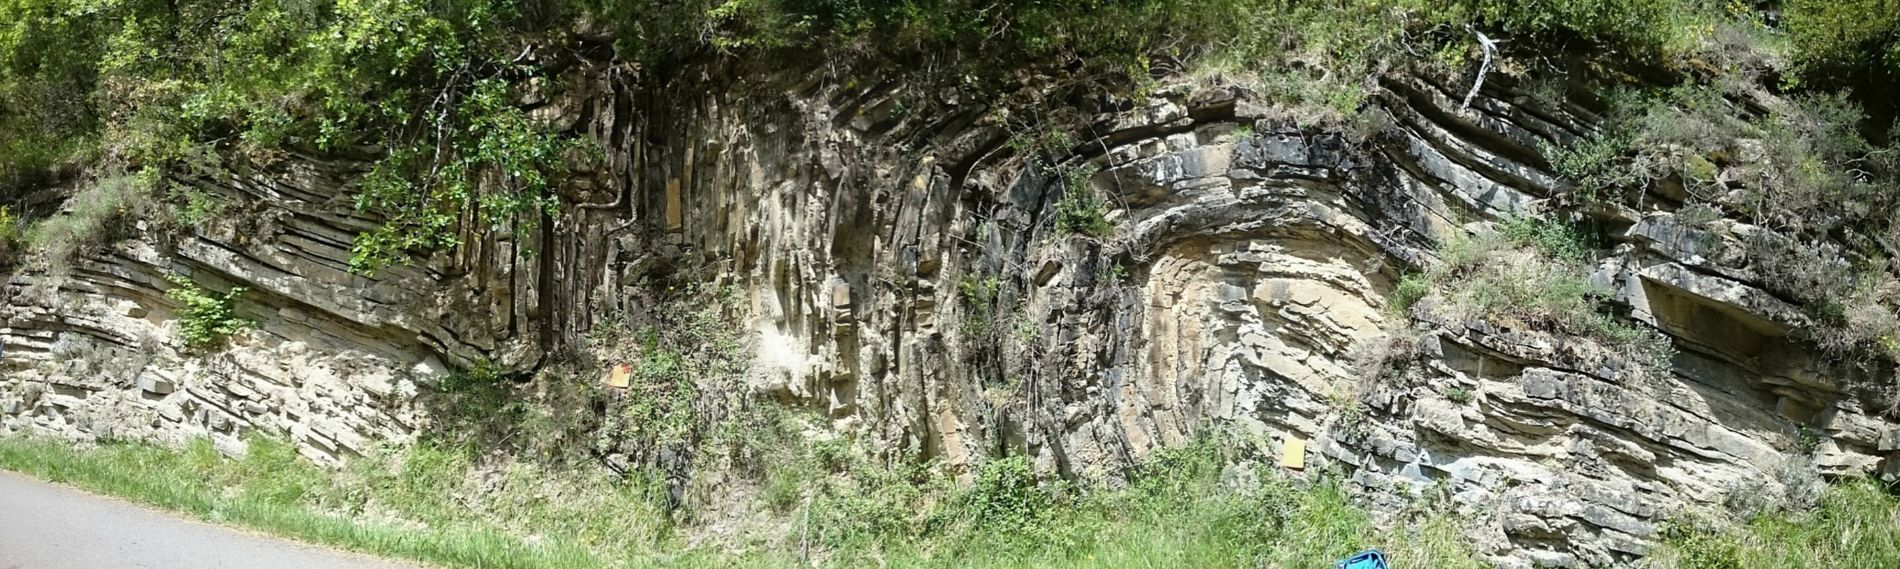
\includegraphics[width=0.8\textwidth]{Hecho1}\\
b & \includegraphics[width=0.8\textwidth]{Hecho2} \\
c & \includegraphics[width=0.8\textwidth]{Hecho3} \\
\end{tabular}
\caption{Folded turbidite lobes outcrop (a) and interpretation with the ``Full'' data set (b) and the ``sparse'' data set (c). 
Tangent and orientation data are shown as black lines and arrows.}
\label{fig:FLH2D}
\end{figure}

The Hecho [het'cho] data set (Fig. \ref{fig:FLH2D}) corresponds to a folded and faulted turbidite outcrop of approximately $16 \times 4$ m located close to Arag\"u\'es del Puerto, Arag\'on, Spain. The layers correspond to Eocene turbidite lobes deposited in the Pyrenean foreland basin (Hecho Group) and then affected by north/south shortening \citep{Bastida2012JSG}. The interbedding of sandstone and shale beds is a source of mechanical heterogeneities which affected the localization of deformation during folding. On this outcrop, most of the shortening is accommodated by flexural slip of sandstone beds; shale beds follow a more ductile deformation between sandstone beds. The fold style (vergence, aperture) changes laterally and vertically, and probably results from variations in the relative thicknesses for the two main rock types. Some minor faults are visible and interpreted on the outcrop. The faults are provided as polygonal lines and triangulated surfaces extrapolated orthogonally 50 cm to the outcrop picture. The mesh resolution of the fault surfaces is approximately 15 cm. The sand lobes only display minor thickness variations at the scale of the outcrop, but some mild apparent thickness variation appears due to perspective. We chose to keep this artifact in the benchmark data set, as thickness variations management challenges have been documented for some implicit structural modeling methods \citep{Laurent2016EaPSL}. 

Nine horizons (H1 to H9) were interpreted on the image plane (XZ) as polygonal lines (Fig. \ref{fig:FLH2D}b). For each of these lines, a random Y coordinate was sampled from a uniform law between -0.5 and 0.5 m to avoid singularities in the three-dimensional case. Some stratal traces and the associated slopes were also obtained by picking some segments parallel to the bedding on the surface. In addition to the ``full'' interpretation, a sparse interpretation is provided to test the ability of the methods to extrapolate away from the data (Fig. \ref{fig:FLH2D}c). This sparse data set only contains the faults and the horizons H1, H2, H4, H5, H7 and H9; only the subhorizontal part of H4 and H5 is provided. As a result, a significant data gap exists at the center of the outcrop between H7 and H2, where the observed layers are overall subvertical.

As some of the implicit modeling methods start with imposed values at the scalar field, we have proposed reference scalar field values (relative geological time) to be equal to a rough estimate of the layer thickness on the interpretation points(Table\ref{tab:Hecho}.

\begin{table}
\centerline{\begin{tabular}{|l|c|c|c|c|c|c|c|c|c|}
\hline
Horizon                       & H1 & H2   & H3 & H4  & H5  & H6 & H7   & H8  & H9  \\
\hline
Scalar value (arbitrary unit) & 0. & 0.78 & 1.15 & 1.9 & 2.5 & 3.1 & 3.9 & 4.4 & 5.2 \\
\hline
\end{tabular}}
\caption{Approximate thicknesses and relative geological time values values chosen for the Hecho Data Set. }
\label{tab:Hecho}
\end{table}

The main goal of this data set is to test the ability of the structural modeling methods to honor conformable series affected by strong and laterally variable folds. 

\subsection{Claudius Data: carbonate mounds from NE Australia}
\label{sec:Claudius}

\begin{figure}
\centering\begin{tabular}{cc}
a & 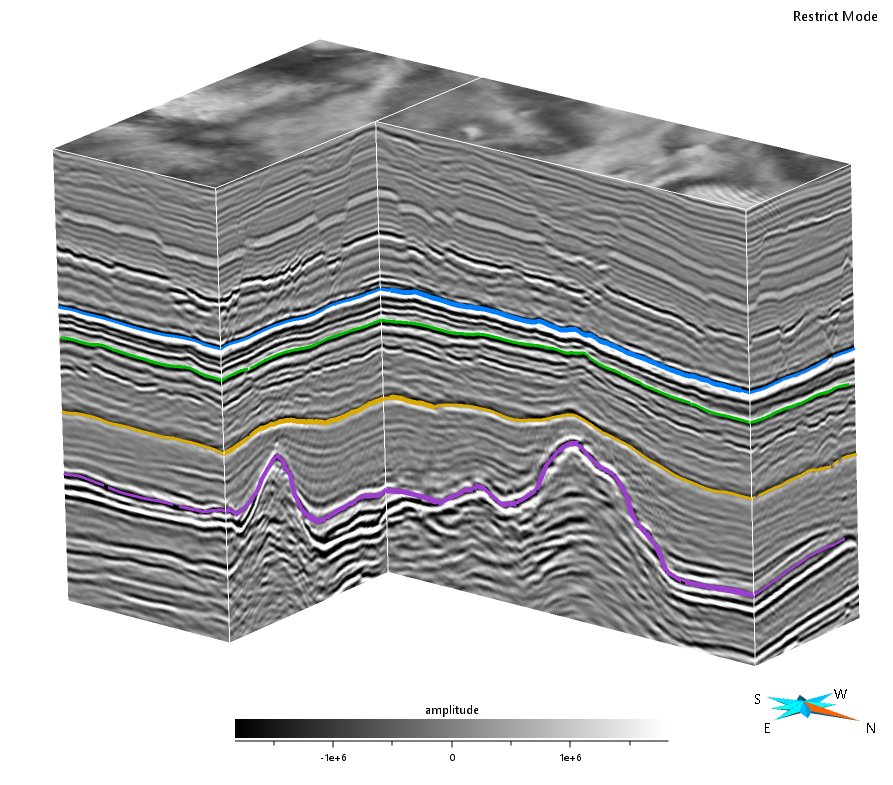
\includegraphics[width=0.7\textwidth,height=6cm]{Claudius}\\
b & 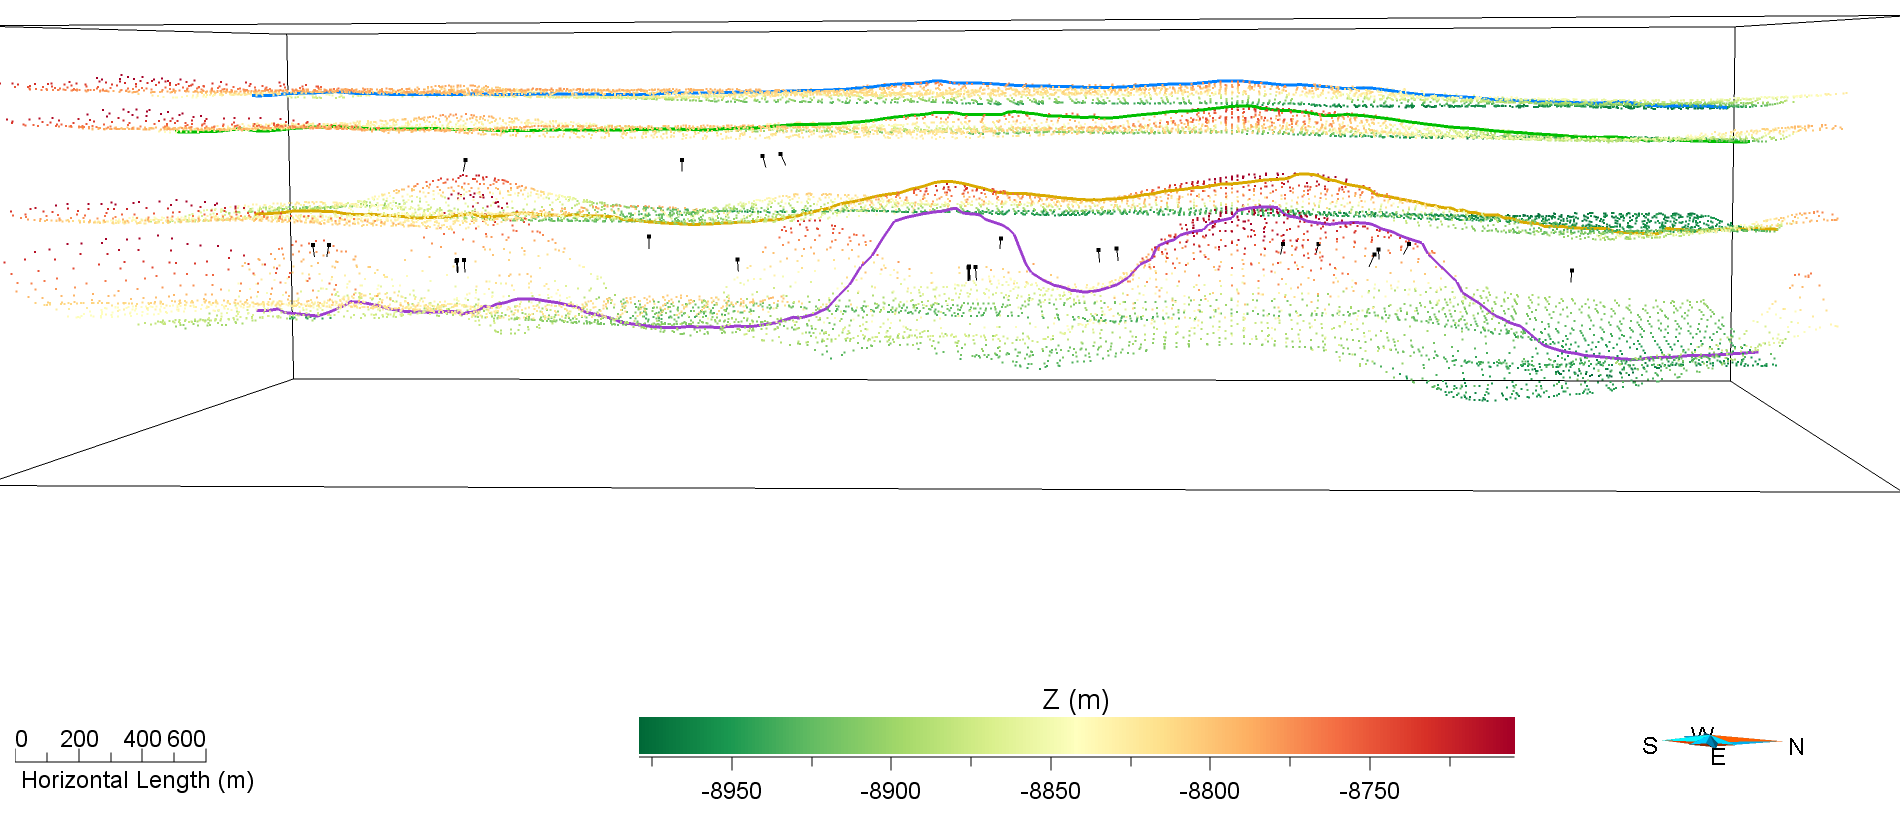
\includegraphics[width=0.8\textwidth]{Claudius1} \\
\end{tabular}
\caption{Interpreted stratigraphic series in the Claudius data set: sections (a) and points in side view (b). A is in blue, B in green, C in yellow and D in violet. In b, the Z Color scale bounds are set for each horizon. Orientation data (normal vectors) in black.}
\label{fig:ClaudiusData}
\end{figure}
\todo[inline]{Add legend and a figure with the reference surfaces and the data only + size details}

The second data set was taken from the offshore Carnarvon Basin, NW Australia. The Claudius area is imaged with a 3D seismic survey acquired by WesternGeco and provided by GeoScienceAustralia. We extracted a small stratigraphic section that displays several carbonate mounds and the associated slope and offshore deposits (Fig. \ref{fig:ClaudiusData}). We interpreted four main horizons named A to D. The most shallow horizon A is relatively flat, whereas D (the top of upper triassic carbonate build-ups) displays significant relief. The intermediate horizons B and C are slightly deformed maybe due to differential compaction. Overall, significant layer thickness variations exist between these stratigraphic surfaces. The detail of the seismic data set shows multiple slope deposits and onlaps, but at the scale of interest, we choose to consider here that the series is globally conformable. The isochore (vertical) thickness of the layer bounded by the C and D seismic reflectors varies between 131~m and 966~m, with an average of 598~m. 

As in the Hecho data set, we did a rough estimate of average layer thicknesses to choose the reference relative geological time values given in Table \ref{tab:Claudius}. Values approximately correspond to the two-way time thickness (in ms) in seismic data. Indeed, the vertical depth coordinate (in meters) was obtained by multiplying by three the two-way seismic travel time (in millisecond). This value corresponds to a very slow medium and is clearly inaccurate, but it allows to easily depth convert the seismic image for testing the results, and to increase the relative thickness variations between the various reflectors.  

\begin{table}
\centerline{\begin{tabular}{|l|c|c|c|c|c|c|c|c|c|}
\hline
Horizon                       & A   & B   & C   & D    \\
Approx. thickness to A (m)    & 0   & 180 & 750 & 1000 \\
\hline
Scalar value (arbitrary unit) & 0 & 60 & 250 & 320      \\
\hline
\end{tabular}}
\caption{Approximate thicknesses and relative geological time values values chosen for the Claudius Data Set. }
\label{tab:Claudius}
\end{table}

The main goal of this data set is to test the ability of implicit methods to model a stratigraphic series having strong thickness variations with one single continuous scalar field. 

\subsection{The Moureze 3D synthetic surface}
\label{sec:Moureze}


\begin{figure}
\centering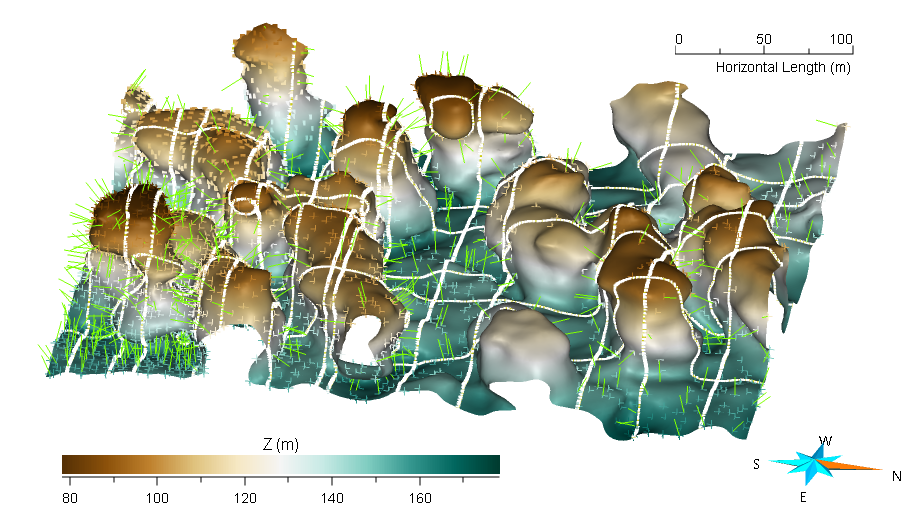
\includegraphics[width=\textwidth]{Moureze}
\caption{Synthetic complex surface generated by a perturbed distance field.}
\label{fig:Moureze}
\end{figure}
\todo[inline]{Add legend and a figure with the reference surfaces and the data only + size details}

To study the behavior of implicit interpolation methods for very complex structural geometries as encountered in salt tectonic studies and ore body delineation, we created a synthetic reference surface using the ODSIM (Object-Distance Simulation) method \citep{Henrion2010MG}. This method was initially introduced to model karsts and hydrothermal alteration bodies \citep{Henrion2008PEIGC,Rongier2014G} and was recently adapted to generate salt surfaces \citep{Clausolles20188ECE2}. In this study, we emulated a hydrothermal alteration body by defining a basement where several subvertical fractures are rooted. The fractures and the basement were defined by manual picking. The distance to the basement and the fracture set was then computed and perturbed by a spatially correlated random field (normal distribution of average 10 m and standard deviation equal to 36 m and Gaussian variogram model of a 36 m horizontal range (isotropic) and 20 m vertical range). Finally, the surface was obtained 
by thresholding (value of 28 m) the perturbed distance field and extracting the surface using Marching Cubes. Some additional cleaning was made to remove isolated bubbles and locally smooth and locally perturb (manually) the obtained geometry. This reference surface is made of one single connected component, but it has three handles. 

From this surface, we extracted two sets of seven E/W and thirteen N/S parallel cross-sections. These sections only contain polygonal lines, some of which consist of several connected components. We also created an unstructured point set by decimating the nodes of the reference surface. The decimation strategy both performed by random sampling and by manual removal of nodes. The manual removal targeted some bumps so that only a very limited number of points remained to constrain the surface geometry. The resulting data points have a heterogeneous density in order to evaluate at once the ability of the reconstruction methods to retrieve the reference shape, both in the case of dense and sparse sampling conditions. A (randomly chosen) fraction of these nodes also provides information about the reference surface orientation. Both the section lines and the points are exactly on the reference surface, so data noise can be considered as negligible. 


\section{Evaluation Metrics}\label{sec:results}

The interpolation results for the various data sets and codes are available at \url{https://github.com/Loop3D/ImplicitBenchmark}.

To evaluate the results, we have considered three aspects: (1) the degree of fit to the input data; (2) the predictivity, considering the fitness to data not included in the benchmark; and (3) intrinsic measures of the produced scalar fields. We will now present and briefly describe and discuss these metrics. 

\subsection{Degree of data fit and predictivity}

All interpolation methods aim at honoring the input data, but we have seen that many methods also approximate the input data. Such approximations allow for filtering geometric noise and are also very useful to avoid spurious extrapolation artifacts. 
Measuring the degree of extrapolation is, therefore, not necessarily bringing much insight in general, as the nugget effect on DcK or the weight of the regularization terms in least-squares or physically based approaches can be tuned to decrease the error. However, this may lead to overfitting and to a lower predictive power of the models away from the data. Therefore, we consider, for each data sets, some test data which can be used to test the ability of the models to predict the structural geometry away from the interpreted points. For this, we consider several types of test data:

\begin{enumerate}
	\item Test points located on the input interfaces allow to test the lateral predictive ability of the various methods.  
  \item Test points located on interfaces not considered in the interpolation data allow to test the ability of implicit modeling to exploit stratigraphic consistency to extrapolate some horizons from others. 
  \item Test orientations, located on data points or not, allow to test the ability of the methods to forecast stratal orientation. 
\end{enumerate}
 
For the test points, computing the root mean squared error between the reference and the interpolated scalar field is possible for all methods. However, for methods that impose the values (Eq. (\ref{eq:datasystem})), the result depends on the initial (and somewhat arbitrary) choice of the initial scala field values. In the increment-based methods, the values can be very different depending on the parameters of the covariance / basis function making any comparison meaningless. Therefore, we have tried to normalize the scalar field by dividing the value difference by the inverse of the local scalar field gradient norm $||\nabla f||$ to approximate a metric error \citep{Caumon2010MG}: 
\begin{equation}
\label{eq:err1}
E_f(\bx_i) = \frac{f_{ref} - f(\bx_i)}{||\nabla f(\bx_f)||},
\end{equation}

\noindent where $\bx_i$ is the test data point location, $f_{ref}$ the reference scalar field value at that location. For result evaluation, we do not necessarily know the reference value. When the gradien norm is locally constant, Eq (\ref{eq:err1}) gives the true distance between the data point and the interpolated level set $f(\bx) = f_{ref}$. However, thickness variations exist in some data sets, so the error $E_f$ may only approximate the distance in that case. Also, there is no such thing as a reference scalar field, so the equation necessarily uses the norm of the interpolated scalar field to assess the error, which introduce another source of error in this error estimation. For these reasons, we finally chose to extract the level set corresponding to reference scalar value and to explicitly compute the error $E_d$ corresponding to the signed distance between the data point and that level set. This computation accurately estimates the true distance, except in some cases when the closest surface points lies on the boundary of the modeling domain. 

This choice can be confirmed by comparing the errors $E_d$ and $Ef$ on the data sets. For example, on the Horizon D of the Claudius data where the gradient varies quite rapidly on some solutions, the relative average distance error between $E_d$ and $Ef$ can be close to 30\% in some cases. 



This is very similar to validation and test data sets in machine learning: 
To present the results, we plan to use a summary table with the main parameters retained for each method and each test case, and explain the rationale about the choice of these parameter values. The modeling results will be put on an open server, together with the scripts and software version information to allow the licensees of each considered software to reproduce the results. 

% \subsection {Consistency}

One of the first questions that want to consider is whether the reconstructed surfaces have the same topology as the reference surfaces. Indeed, implicit methods do not \textit{a priori} impose a particular topology for the implicit surfaces. This is a very interesting feature, for instance in the case of the Moureze data, as arbitrary topology can emerge from the data. However, bubbles should not appear when modeling layered strata, even in the case of sparse sampling or of strong thickness variations. 

% \subsection{Accuracy}

The second criterion concerns the accuracy of the interpolation. This should be a relatively easy case, as all methods generally have a parameter controlling the degree of data fit (e.g., the constraint weight in DSI or the variogram nugget effect in DcK). As not all methods use the same iso-values $f_k$, we plan to perform a projection of the points onto the reconstructed surfaces, and then check for possible bias (average of the signed distance) and error (variance of the deviation and maximum deviation corresponding to the Hausdorff distance). 

The third criterion will be to check the spatial forecasting ability, by checking the reconstructed surfaces against the reference geometries. This will be performed not only globally, but also in some targeted locations where data gaps were purposely introduced in the data set. In conjunction with the data accuracy, this should allow to test the ability of methods to predict some ``unseen'' features using the same data configuration, considering in particular the ability to extrapolate a horizon away from the data points laterally and orthogonally to the stratigraphy. Depending on the data configuration, it is likely that the regularization term might play a positive or adverse role there. In particular, when geological concepts and knowledge are incorporated as model parameters \citep[e.g.,][]{Laurent2016EaPSL,Grose2017JSG,Grose2018JGRSE,Grose2019JoSG} and when the choice of these model parameters is appropriate, it is possible to improve the predictive ability of models. Therefore, we also need to account for the number of method parameters and how they are infered and not just bluntly judge a method's performance based on RMS errors on some particular test data.  

Last, we also would like to provide some performance metrics about the various steps of the algorithms (domain construction, interpolation \textit{sensu stricto}, and isosurface visualization / extraction). A particular difficulty in this performance study will be to make sure that performance comparisons are sensible in spite of the probable use of different hardware configurations by the various co-authors. 

%\subsection{Performance}
 
\todo[inline]{Discuss about performance issues. This could be challenging, as everyone will run tests on a different machine, and codes have very different features (parallel or not, 2D or 3D). Scalability can be compared nonetheless by fitting a law regression between the number of points and the computational time. THis would call for everyone to apply the interpolation with decimated data sets (e.g. using 1/100, 1/50, 1/10, 1/5, 1/2 of the points)... The time ratio between model preparation (e.g., meshing), interpolation (solving the system) and visualization (marching cubes or the like) could also be considered. }


\section*{Discussion and conclusions}
\label{sec:conclu}
We have proposed three data sets that can be used to assess the ability of implicit structural modeling methods to build relatively complex geological surfaces in the presence of sparse data. These data sets were designed to test both two-dimensional and three-dimensional implicit modeling codes. They are heterogeneous in size and in types of geological features, showing a highly conformable but strongly folded stratigraphic series, sedimentologically-controlled mini-basins involving fast changes of lateral stratigraphic thickness, and a complex fracture-controlled hydrothermal surface. 

We briefly reviewed the existing implicit modeling methods, which are currently being confronted to the benchmark data sets by the co-authors of this paper. Finally, we discussed about the criteria we intend to use to evaluate the benchmark results. 
Overall, we hope that these results will contribute to identifying avenues for further research in three-dimensional structural modeling, and that the proposed data can be used for testing future methods in the future. We welcome comments and suggestions for this work in progress. 

\section*{Acknowledgments}

This work was performed in the frame of the LOOP project (\url{https://loop3d.org/}) and the RING project (http://ring.georessources.univ-lorraine.fr/). We would like to thank for their support the industrial and academic sponsors of the RING-GOCAD Consortium managed by ASGA, and the LOOP project partners. We would also like to thank Geoscience Australia for providing the Claudius seismic data set and Emerson for the SKUA-GOCAD software used to prepare the data. 

% Set your bibliography file here (without .bib)
\bibliography{biblio}

\end{document}

%------------------------------------------
